\documentclass[a4paper,11pt]{article}
\usepackage{geometry,gretlhds}
\usepackage{url,fancyvrb}
\usepackage{pifont}
\usepackage[utf8]{inputenc}
\usepackage[pdftex]{graphicx}
\usepackage{color}
\usepackage{dcolumn,amsmath,mathrsfs}
\usepackage{natbib}
\bibliographystyle{gretl}

\graphicspath{{graphs/}}

\newenvironment{funcdoc}[1]
{\noindent\hrulefill\newline\texttt{#1}\par\noindent\hrulefill\par\medskip\par}
{\bigskip}

% ---------- Ripped from gretl.sty ----------------------------------------

\newcommand{\scriptname}{Example}

\newcommand{\app}[1]{\textsf{#1}}
\newcommand{\cmd}[1]{\texttt{#1}}
\newcommand{\varname}[1]{\texttt{#1}}
\newcommand{\option}[1]{\texttt{-{}-#1}}

\newcommand{\ttsl}[1]{\ttfamily{\textsl{#1}}\normalfont}

\newenvironment{textcode}{\par\small\ttfamily}
{\normalfont\normalsize\par}

\DefineVerbatimEnvironment%
{code}{Verbatim}
{fontsize=\small, xleftmargin=1em}

\DefineVerbatimEnvironment%
{scode}{Verbatim}
{frame=lines, framesep=2ex, fontsize=\small,
 formatcom=\color{myteal}, rulecolor=\color{mygray}}

\DefineVerbatimEnvironment%
{scodebit}{Verbatim}
{fontsize=\small, formatcom=\color{myteal}}

\DefineVerbatimEnvironment%
{scodebot}{Verbatim}
{frame=bottomline, framesep=2ex, fontsize=\small,
 formatcom=\color{myteal}, rulecolor=\color{mygray}}

\renewcommand{\arraystretch}{1.2}

\definecolor{mygray}{rgb}{0.85,0.85,0.85} 
\definecolor{myteal}{rgb}{0.0,0.25,0.15} 

\def\floatpagefraction{.8}

%% add script as float (Example)
\newcounter{script}[section]
\renewcommand \thescript
     {\ifnum \c@chapter>\z@ \thechapter.\fi \@arabic\c@script}
\def\fps@script{tbp}
\def\ftype@script{1}
\def\ext@script{los}
\def\fnum@script{\scriptname\nobreakspace\thescript}
\newenvironment{script}
               {\@float{script}}
               {\end@float}
\newenvironment{script*}
               {\@dblfloat{script}}
               {\end@dblfloat}
\newcommand\theHscript{\thechapter.\arabic{script}}

\newcommand{\tip}[1]{\par\vspace{4pt}
 \ding{43} {\small \sffamily #1}\par\smallskip}

% ---------- End rip ------------------------------------------------------

\newcommand{\stdu}{\ensuremath \varepsilon}
\newcommand{\uhat}{\ensuremath u}
\newcommand{\InfSet}[1]{\ensuremath \mathcal{F}_{#1}}
\newcommand{\IRF}[1]{\ensuremath \mathcal{I}_{#1}}
\newcommand{\FEVD}[1]{\ensuremath \mathcal{VD}_{#1}}
\newcommand{\pder}[2]{\ensuremath\frac{\partial #1}{\partial #2}}
\DeclareMathOperator{\VEC}{\mathrm{vec}}

\newcommand{\gig}{\texttt{gig}}

\title{The \gig\ package}
\author{Jack Lucchetti \and Stefano Balietti}
\date{version 2.2}
\begin{document}

\maketitle

\begin{abstract}
The \gig\ package is a collection of \app{gretl} scripts to estimate
univariate conditional heteroskedasticity models. What is described
here is \gig\ version 2.0, which is substantially different from the
previous version: it makes use of several new \app{gretl} features and
is totally incompatible with the old version. In return, you get a
package that is considerably simpler to use, maintain and extend and
integrates in a much smoother way with the \app{gretl} GUI.
\end{abstract}

\tableofcontents

\section{Introduction}

A general description of the models that \gig\ can handle can be given
by the following system:
\begin{eqnarray}
  \label{eq:meaneq}
  E_{t-1}(y_t) & = & \pi'x_t \\
  \label{eq:espdef}
  \uhat_{t} \equiv y_t - E_{t-1}(y_t) & \Longrightarrow &
  y_t = \pi'x_t + \uhat_{t} \\
  \label{eq:vareq}
  h_t \equiv V_{t-1}(\uhat_{t}) & = & 
  v(\uhat_{t-1}, \uhat_{t-2}, \ldots, 
  h_{t-1}, h_{t-2}, \ldots, z_t) \\
  \label{eq:stdinn}
  \stdu_t & = & \frac{\uhat_{t}}{\sqrt{h_t}}
\end{eqnarray}
which could be read as follows: it is assumed (eq.~\ref{eq:meaneq})
that the conditional expectation\footnote{Of course, all the relevant
  moments are supposed to exist.} of an observable variable $y_t$ to an
information set\footnote{We could be more rigorous and impress the
  reader with $\sigma$-algebras and filtrations, but we can't be
  bothered, ok?}  $\InfSet{t-1}$ (denoted as $E_{t-1}$) is a linear
function of quantities known at time $t-1$. Clearly, the information
set may contain exogenous variables as well as lags of $y_t$, which
are all collected in the vector $x_t$. This makes it possible to write
an equation (eq.~\ref{eq:espdef}) for the conditional mean of $y_t$.

As for the conditional variance (eq.~\ref{eq:vareq}), this is assumed
to be a known function, with possibly also some observable exogenous
variables $z_t$. The most basic choice is the GARCH model, in which
\eqref{eq:vareq} specialises to
\[
  h_t = \omega +  \sum_{i=1}^q \alpha_i \uhat_{t-i}^2 + 
  \sum_{j=1}^p\beta_j h_{t-j} ,
\]
but a number of exotic alternatives have been devised in the past 30
years (see section \ref{sec:models}). Note that the conditional
variance, as specified in eq.~\eqref{eq:vareq}, may or may not contain
exogenous explanatory variables, but a constant term must always be
present (\gig\ adds one automatically otherwise). The
standardised innovations $\stdu_t$ are trivially defined by
eq.~\eqref{eq:stdinn}, and have zero conditional mean and unit
conditional variance by construction.

\tip{\emph{Nota bene}: the convention used in the previous version of \gig\
was to use the letter $p$ to indicate the ARCH order and $q$ for the
GARCH order, which was inconsistent with \app{gretl} itself and, most
importantly, with \cite{Bollerslev-86}. \textbf{This is now reversed},
so $p$ is the GARCH order and $q$ is the ARCH order.}


The parameters of these models are almost invariably estimated via
maximum likelihood (or pseudo-ML), which brings up the subject of a
suitable choice for the conditional distribution of $\stdu_t$.  This has
also been the object of much speculation, given the need to
accommodate several stylised facts, such as leptokurtosis:
\gig\ provides algorithms for the most popular choices in the
applied literature (see Table \ref{tab:densities}).

\begin{table}[hptb]
  \centering
  \begin{footnotesize}
  \begin{tabular}{p{0.275\textwidth}cr}
    \hline 
    \textbf{Name} &  \textbf{Density}  &  \textbf{Parameters} \\
    \hline 
    \\
    Normal & 
    $\frac{1}{\sqrt{2\pi h_t}} 
    \exp \left\{-\frac{\stdu_t^2}{2}\right\}$ & 
    none \\
    Student's $t$ & 
    $\frac{K(\nu)}{\sqrt{h_t}}
    \left[1+\frac{\stdu_t^2}{\nu-2}\right]^{-(\nu + 1)/2}$ &
    $\nu > 2$ \\
    Generalised Error Distribution (GED) &
    $C(\nu)\exp\left\{-\left|\frac{\stdu_t}{\kappa_\nu}\right|^\nu\right\}$
    & $\nu > 0$ \\
    Skewed $t$ & 
    $\frac{b K(\nu)}{\sqrt{h_t}}
    \left[1 + \frac{\zeta_t^2}{\nu - 2}\right]^{-(\nu + 1)/2}$ 
    & $\nu > 2, \xi \in \Re$ \\
    \\
    Skewed GED &
    $\left\{
      \begin{array}{cc}
        D(\nu) \exp\left\{-\beta_1 \left|\stdu_t - m\right|^\nu\right\} &
          \stdu_t < m \\
        D(\nu) \exp\left\{-\beta_2 \left|\stdu_t - m\right|^\nu\right\} &
          \stdu_t \ge m 
      \end{array}
    \right.$
    & $\nu > 0, \xi \in \Re$ \\
    \\
    \hline
    \hline
  \end{tabular}
  \end{footnotesize}

\begin{eqnarray*}
  K(\nu) & = &
  \frac{\Gamma\left[(\nu + 1)/2\right]}  {\sqrt{\pi (\nu - 2)}\Gamma(\nu/2)} \\
  C(\nu) & = &
  \frac{\nu}{2}\sqrt{\frac{\Gamma(3/\nu)}{\Gamma(1/\nu)^3}} \\
  \kappa_\nu & = &
  \sqrt{2^{-\frac{2}{\nu}}\frac{\Gamma(1/\nu)}{\Gamma(3/\nu)}} \\
  a & = & K(\nu) \cdot 4 \lambda  \left( \frac{\nu - 2}{\nu - 1} \right) \\
  b & = & \sqrt{1 + 3\lambda^2 - a^2} \\
  \lambda & = & \tanh(\xi) \\
  \zeta_t & = & \left\{
    \begin{array}{ll}
        \frac{b \stdu_t + a}{1-\lambda} & \mathrm{for\ } \stdu_t < -a/b \\
        \frac{b \stdu_t + a}{1+\lambda} & \mathrm{for\ } \stdu_t > -a/b
      \end{array}
      \right. \\
  D(\nu) & = & 
  \frac{1}{\Gamma(1/\nu)}\sqrt{\frac{\Gamma(3/\nu)}{2 \cdot \Gamma(1/\nu)}
  \left(\frac{1 + \lambda}{1 - \lambda}\right)^3 - 
  \left(2 \lambda \Gamma(2/\nu)\right)^2 } 
\end{eqnarray*}
  \caption{Conditional densities for $\stdu_t$}
  \label{tab:densities}
\end{table}

A brief remark on the skewed distributions: compared to their original
parametrisation, we treat $\lambda$ as the hyperbolic tangent of an
unconstrained real parameter $\xi$; this reparametrisation is
inconsequential in substance, but very helpful numerically.

\section{The models}
\label{sec:models}

\subsection{The APARCH Family}
\label{sec:APARCH}

Most of the models \gig\ can handle can be thought of as special
cases of the Asymmetric Power ARCH (APARCH) model, introduced by
\cite{Ding-Engle-Granger}. This model is able to accommodate
asymmetric effects and power transformations of the variance. Its
specification for the conditional variance is the following:
\begin{equation} \label{eq:aparch} \sigma_t^\delta = \omega'z_t +
  \sum_{i=1}^q \alpha_i(|\uhat_{t-i}| - \gamma_i
  \uhat_{t-i})^\delta + \sum_{j=1}^p\beta_j\sigma_{t-j}^\delta
\end{equation}
where $\sigma_t \equiv \sqrt{h_t}$, the parameter $\delta$ (assumed
positive, but typically ranging between 1 and 2) performs a Box-Cox
transformation and $\gamma$ captures the asymmetric effects.  Special
values of the parameters give rise to the special cases enumerated in
Table \ref{tab:APARCH-submodels}.

\begin{table}[hptb]
  \centering
  \begin{tabular}{p{0.2\textwidth}p{0.3\textwidth}p{0.4\textwidth}}
    \hline
    MODEL & AUTHOR & CONSTRAINTS \\
    \hline
    \textbf{ARCH} & \cite{Engle-82} & $\delta=2$, $\gamma_i = 0$ for
 $ i=1,\ldots,q$ and $\beta_j = 0$ for $j=1,\ldots,p$ \\
 \hline
 \textbf{GARCH} & \cite{Bollerslev-86} & $\delta=2$,
  $\gamma_i = 0$ $ i=1,\ldots,q$ \\
  \hline
  \textbf{Taylor/Schwert GARCH} & \cite{Taylor} and \cite{Schwert} & $\delta=1$,
  $\gamma_i = 0$ $ i=1,\ldots,q$\\
  \hline
  \textbf{GJR} & \cite{Glosten-Jagannathan-Runkle} & $\delta=2$ \\
  \hline
  \textbf{TARCH} & \cite{Zakoian} & $\delta=1$\\
  \hline
  \textbf{NARCH} & \cite{Higgins-Bera} & $\gamma_i = 0$ for
  $ i=1,\ldots,p$ and $\beta_j = 0$ for $j=1,\ldots,p$\\
  % \hline
  % \textbf{Log-ARCH} & \cite{Geweke} and \cite{Pantula} & if
  % $\delta \rightarrow 0$.\\
  \hline  
  \end{tabular}
  \caption{APARCH nested sub-models}
  \label{tab:APARCH-submodels}
\end{table}

The GJR model is given a special treatment in \gig. Other software
packages adopt a different, albeit equivalent, parametrisation for the
same model (some programs even call it by some other name). What \gig\
considers to be the GJR model
\begin{equation} \label{eq:GJR-gig} \sigma_t^2 = \omega'z_t +
  \sum_{i=1}^q \alpha_i(|\uhat_{t-i}| - \gamma_i
  \uhat_{t-i})^2 + \sum_{j=1}^p\beta_j\sigma_{t-j}^2
\end{equation}
is sometimes reparametrised as
\begin{equation} \label{eq:GJR-eviews} \sigma_t^2 = \delta'z_t +
  \sum_{i=1}^q \left( \alpha_i \uhat_{t-i}^2 + \gamma_i d_{t-i}
  \uhat_{t-i}^2 \right) + \sum_{j=1}^p\beta_j\sigma_{t-j}^2
\end{equation}
where $d_t = 1$ if $\uhat_{t}<0$ and 0 otherwise. The correspondence
between the two sets of parameters is left as an exercise to the
reader. An example will be given in section \ref{sec:GUI}.

In order to facilitate comparisons, when you estimate a GJR model,
\gig\ will print out both forms. However, only the parameters
corresponding to \eqref{eq:GJR-gig} will be saved.

\subsection{The EGARCH model}
\label{sec:EGARCH}

The Exponential GARCH (EGARCH) model, put forward by \cite{Nelson}, is
the only model presently available in \gig\ that is not nested
in the APARCH model. This is because eq.~\eqref{eq:vareq} is written
in terms of the logarithm of the variance instead of the variance
itself. Moreover, it captures asymmetric effects as a function of the
standardised innovations. The log-conditional variance $\ln(h_t)$ is
thus given by:
\begin{equation}\label{eq:egarch-0}
  \ln h_t = \bar{\omega}'z_t  + 
  \sum_{i=1}^q \left[
    \alpha_i \left( |\stdu_{t-i}| - \sqrt{2/\pi}\right) + \gamma_i \stdu_{t-i}
  \right]+
  \sum_{j=1}^p \beta_j \ln(h_{t-j})
\end{equation}

However, this is not the exact form that \gig\ uses: there are some
computational advantages in moving the term $\sqrt{2/\pi}$ out of the
summation operator. The model actually estimated is
\begin{equation}\label{eq:egarch}
  \ln h_t = \omega'z_t  + 
  \sum_{i=1}^q \left( \alpha_i |\stdu_{t-i}| + \gamma_i \stdu_{t-i} \right)+
  \sum_{j=1}^p \beta_j \ln(h_{t-j})
\end{equation}
where the element of the vector $\omega$ corresponding to the constant
equals the corresponding term of $\bar{\omega}$ minus $\sqrt{2/\pi}
\cdot \sum_{i} \alpha_i$.

Note that the sign of the asymmetric component in the APARCH and
EGARCH models do not match (compare equations \eqref{eq:aparch} and
\eqref{eq:egarch}). This is rather unfortunate, since it means that
the parameter $\gamma$ must be given an opposite interpretation in the
two cases. However, we decided to keep the two formulations
inconsistent for compatibility with other software packages.

% It is worthwhile to point out that, as E[ln($h_t$)] $\neq$
% ln(E[$h_t$]), the EGARCH is thought to analyze the logarithm of the
% conditional variance, rather than the conditional variance itself,
% which can be estimated as follows:

% \begin{align}\label{eq:egarch-3}
%   h_t & = \hat{\zeta}^*\sum_{j=1}^q(\hat{h}_{t-j}^{\hat{\beta}})
%   \exp(\sum_{i=1}^p
%   \frac{\hat{\alpha_i}|\uhat_{t-i}|+\hat{\phi}_i
%     \uhat_{t-1}}{\sqrt{\hat{h}_{t-i}}})
%   \intertext{where}
%   \zeta^* & = \exp(\zeta - \sum_{i=1}^p \alpha_i\sqrt{\frac{2}{\pi}})
% \end{align}


\section{How you do things}

The central idea in \gig\ is that your model is contained in a
\app{gretl} bundle\footnote{If you don't know what a bundle is in
  \app{gretl}, you may want to have a look at the User's Guide,
  chapter 11. In short, a bundle is a container for assorted objects,
  such as matrices, series etcetera.}, which is set up first with the
basic information about the model (what the dependent variable is,
what kind of model it is, and so on), and then filled with all the
quantities available after estimation (coefficients etc).

Like most statistical procedures that come with \app{gretl}, there are
two ways to accomplish the above: either you use a graphical
interface, which is very intuitive and easy to use, or you use a
script, which is more awkward at the beginning, but gives you more
power and flexibility.

In this section, we will look at a few examples. We will assume that
\gig\ is installed correctly as a \app{gretl} addon and that you
already have a certain degree of familiarity with \app{gretl}'s
interface and scripting syntax.


\subsection{The GUI way}
\label{sec:GUI}

Suppose you have already loaded the data you want to analyse, and have
already performed the necessary preliminary data transformations, if
any. For example, suppose you loaded the example \app{gretl} dataset
called \texttt{djclose}, and already have created a variable called
$y_t$ which contains the daily returns, that is 
\begin{code}
  series y = 100 * ldiff(djclose)
\end{code}
If you plot $y_t$, you'll see the typical financial time series plot,
with the volatility clustering and all the other famous ``stylised
facts'':
\begin{center}
  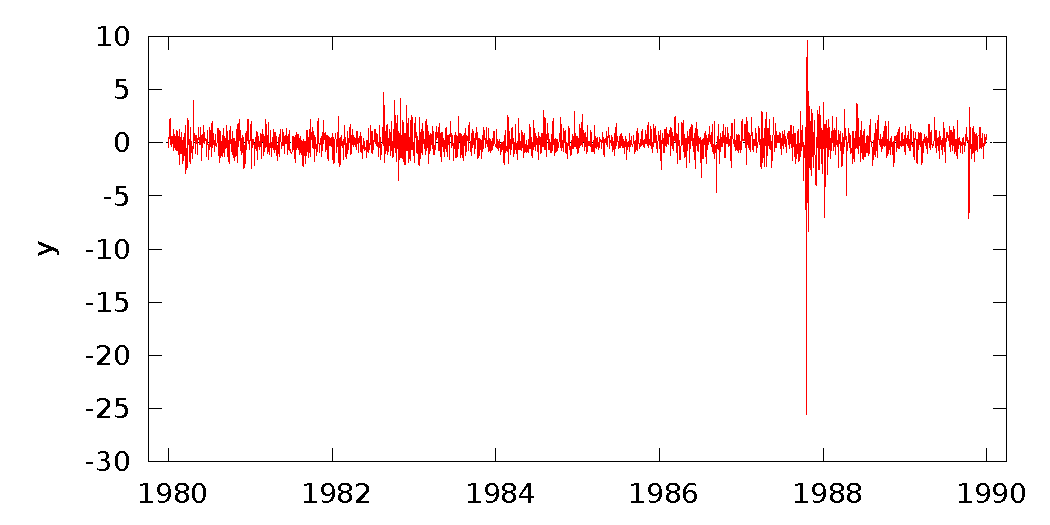
\includegraphics[width=0.75\textwidth,height=0.35\textwidth]{graphs/djret}
\end{center}

The GUI hook to \gig\ can be found under the \emph{Model $>$ Time
  Series $>$ GARCH variants} heading. By choosing it you'll be
presented with a window similar to the one shown in Figure
\ref{fig:GUI-gig}. The meaning of the various element should be rather
clear, except perhaps for a few that require some explanation.

\begin{figure}[htb]
  \centering
  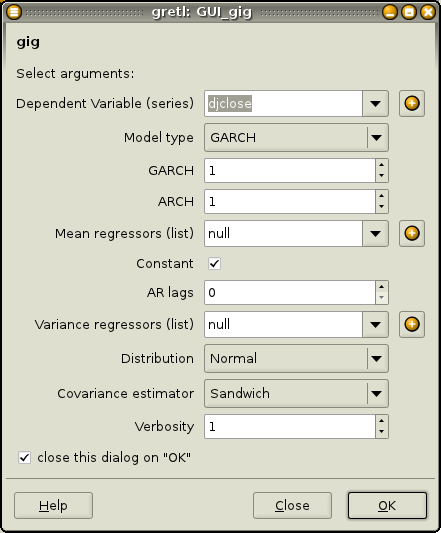
\includegraphics[scale=0.45]{graphs/GUI-gig}
  \caption{GUI hook for \gig}
  \label{fig:GUI-gig}
\end{figure}

\begin{description}
\item[The regressors lists] These are two lists holding the exogenous
  variables in the conditional mean ($x_t$ in equation
  \ref{eq:meaneq}) and conditional variance equation ($z_t$ in
  equation \ref{eq:vareq}), respectively. They both default to
  \texttt{null}, an empty list, although in the variance regressors
  list a constant term is automatically included if absent. If some
  lists are already defined, you can pick them from the list;
  alternatively, you can create lists on the fly by using the ``+''
  button.  Note that, from version 1.9.3 of \app{gretl} onwards, you
  can use a single series in lieu of a list proper, so for example if
  you want a constant to appear in your conditional mean, you may just
  type \texttt{const} in the ``mean regressors'' text box.

  Note, however, that you you have two separate GUI elements for
  including in your mean specification the most common choices, that
  is a constant term and/or lags of the dependent variable. Hence,
  you'll need to specify the mean regressors only if you have mean
  terms other than those (for example, a time trend or some other
  exogenous variable).

\item[Covariance estimator] Here you can choose between 3 algorithms
  for computing the variance-covariance matrix of the estimated
  parameters. Sandwich (also known as QMLE: see \cite{bolwoo92}) is
  the default, but OPG is the fastest.
\item[Verbosity] An integer, ranging from 0 to 2: the default is 1,
  which means you want to see the estimated model. If you choose 0,
  you see nothing (all results can be retrieved later); if you choose
  2, you get to see the BFGS iterations, which may be helpful in some
  cases, especially when the algorithm fails to converge (see also
  section \ref{sec:numerical}).
\end{description}

Now suppose that we want to estimate a GJR(1,1) model with a constant
as mean regressor and the $t$ distribution as the density for the
standardised innovations $\stdu_t$. In practice, the following model:
\begin{eqnarray*}
  y_t & = & \mu + \uhat_{t} \\
  h_t \equiv V_{t-1}(\uhat_{t}) & = & \omega +
  \alpha(|\uhat_{t-1}| - \gamma \uhat_{t-1})^2 + \beta h_{t-1} \\
  f(\stdu_t | \InfSet{t-1}) & = & \frac{K(\nu)}{\sqrt{h_t}}
    \left[1+\frac{\stdu_t^2}{\nu-2}\right]^{-(\nu + 1)/2}
\end{eqnarray*}

\begin{figure}[htb]
  \centering
  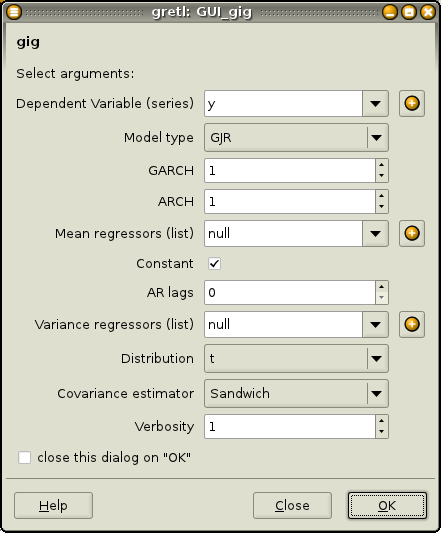
\includegraphics[scale=0.45]{graphs/GUI-gig-GJR}
  \caption{GUI hook for \gig\ (GJR example)}
  \label{fig:GUI-gig-GJR}
\end{figure}

All you have to do is select the appropriate entries in the
\texttt{GUI\_gig} window. When it looks like Figure
\ref{fig:GUI-gig-GJR}, just press OK\footnote{Note a subtle difference
  between Figure \ref{fig:GUI-gig} and Figure
  \ref{fig:GUI-gig-GJR}. In the latter, the ``close this dialog'' tick
  box near the bottom is not ticked. This, of course, has no effect on
  the estimates, but may be quite handy if you want to revise your
  model interactively.} and, after a second or two, the following
estimate should appear\footnote{Note that the GJR model is presented
  with both parametrisations discussed in section
  \ref{sec:APARCH}.}. The asterisk at the end of the first line of the
output indicates that the analytical score was used for estimation.:

\begin{code}
Model: GJR(1,1) [Glosten et al.] (Student's t)*
Dependent variable: y
Sample: 1980/01/03-1989/12/29 (T = 2527), VCV method: Robust

    Conditional mean equation

             coefficient   std. error     z     p-value
  -----------------------------------------------------
  const       0.0483897    0.0170808    2.833   0.0046  ***

    Conditional variance equation

             coefficient   std. error      z      p-value
  -------------------------------------------------------
  omega       0.0249070    0.00890124    2.798    0.0051  ***
  alpha       0.0332144    0.00895699    3.708    0.0002  ***
  gamma       0.0259622    0.108140      0.2401   0.8103 
  beta        0.939891     0.0155313    60.52     0.0000  ***

   (alt. parametrization)

             coefficient   std. error      z      p-value 
  --------------------------------------------------------
  delta      0.0249070     0.00890123    2.798    0.0051   ***
  alpha      0.0315122     0.00726215    4.339    1.43e-05 ***
  gamma      0.00344928    0.0149219     0.2312   0.8172  
  beta       0.939891      0.0155313    60.52     0.0000   ***

    Conditional density parameters

             coefficient   std. error     z     p-value 
  ------------------------------------------------------
  ni           5.54597      0.738486    7.510   5.92e-14 ***

	Llik:  -3408.87517	 AIC:   6829.75034
	BIC:    6864.75906	 HQC:   6842.45322
\end{code}

In fact, the estimate above will be contained in a window on top of
which you get several icons: the most interesting are
\begin{description}
\item[a ``Save'' icon] Use this to save the output as text or to store
  the model bundle as a gretl icon for later use.
\item[a ``Save bundle content'' icon] If you click here, you will see
  a list of all the objects contained in the bundle holding your
  model. A complete list is available as Appendix
  \ref{sec:bundle_struct}, but most names should be
  self-explanatory. This is where you retrieve stuff for later
  processing. You also have the option (on top) of saving the whole
  bundle as such, for later processing.\footnote{In fact, at this
    stage, the bundle will already be in the Icon View with a
    temporary name. Do we want to advertise this or should we let the
    user discover this little trick by himself?} For example, suppose
  that you want to save the standardised residuals. From the
  \emph{Save} menu, just pick the \emph{stduhat} entry. A dialog
  similar to the one shown in Figure \ref{fig:GUI-saveres} should
  appear: just give the series any time you want and, optionally, a
  description. For example, you can choose ``\texttt{e}'' as the
  series name and on ``Estimated standardised residuals'' as the
  description. The series \texttt{e} should now appear in your main
  \app{gretl} window, so you can plot it, analyse it, save it
  etcetera.

\item[a ``Graph'' icon] By clicking here, you can choose for a plot to
  display: the choice is between a ``Time series'' plot and a
  ``Density'' plot. For more details on the nature of these plots, see
  section \ref{sec:plots}. To edit and/or save those plots, just
  right-click on them.
\end{description}

\begin{figure}[htb]
  \centering
  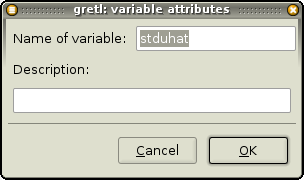
\includegraphics[scale=0.5]{graphs/GUI-saveres}
  \caption{GUI window for saving bundle elements}
  \label{fig:GUI-saveres}
\end{figure}

% \begin{figure}[htb]
%   \centering
%   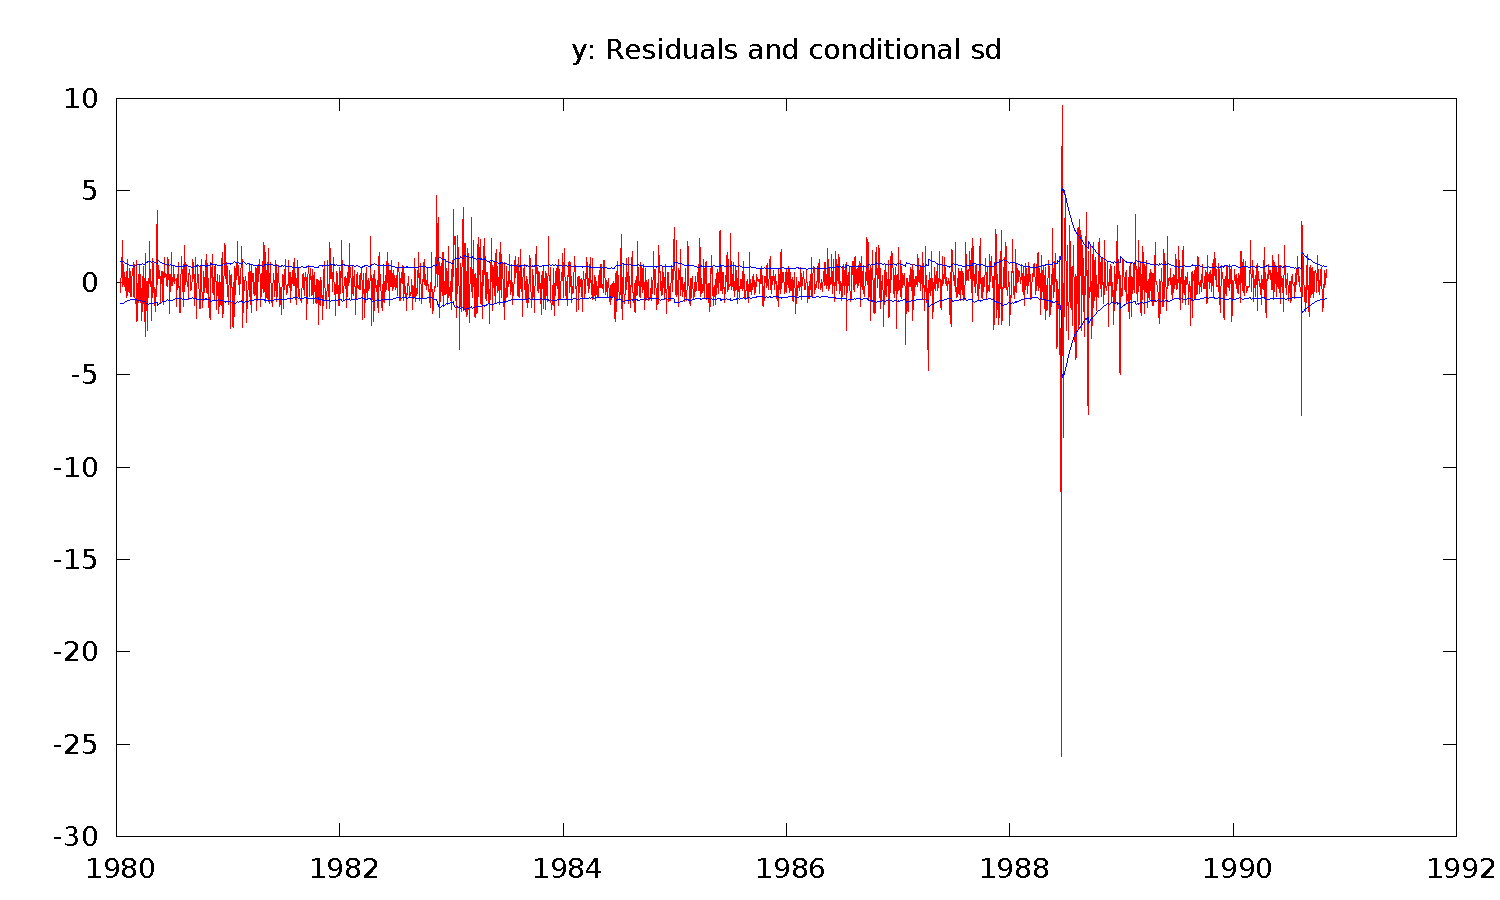
\includegraphics[scale=0.5]{graphs/ts-plot-gjr}
%   \caption{Post-estimation time series plot (GJR example)}
%   \label{fig:ts-plot-gjr}
% \end{figure}


\subsection{Scripts: a plain-vanilla GARCH}
\label{sec:plain-garch}

The typical way to use \gig\ from a script is to break the sequence of
operations implicit in the GUI call in a series of steps. This will
(hopefully) help you write nice, tidy, modular and reusable scripts.

The two functions that you cannot avoid using are called
\texttt{gig\_setup} and \texttt{gig\_estimate}: the former creates a
bundle with the basic info about your model, the latter populates it
with the estimates. The GUI interface merges these two actions into
one, but when you work from a script keeping the two separate has its
pros.

To give you a very simple example of the way the two functions work,
we will estimate the most basic GARCH model, that is one in which
equations \eqref{eq:espdef} and \eqref{eq:vareq} specialise to
\begin{eqnarray*}
  y_t & = & \uhat_{t} \\
  h_t & = & \omega + \alpha \uhat_{t-1}^2 + \beta h_{t-1}
\end{eqnarray*}
and the conditional distribution of $\uhat_{t}$ is assumed to be
normal, that is $\uhat_{t} | \InfSet{t-1} \sim N(0, h_t)$.

The corresponding script reads as follows:
\begin{code}
# Import the gig library
include gig.gfn

# Read the data and compute returns
open djclose
y = 100*ldiff(djclose)

# Estimate a plain-vanilla GARCH model
plato = gig_setup(y)
gig_estimate(&plato)
\end{code}

The first function we use is \texttt{gig\_setup}: this function
creates a bundle (called \texttt{plato} in the present example), which
contains the basic information on the model that are needed for
estimation, that is the dependent variable, the model type and the
regressors for the mean and variance equations. In this case, however,
the only parameter we need to pass to the function needs is the name
of the series containing $y_t$. This is because \texttt{gig\_setup}
has several default options that allow you to omit some arguments in
certain cases. Since in this example the model for the conditional
variance is GARCH (the default) and there are no exogenous regressors
either in the mean equation nor in the variance equation, you may just
omit the corresponding parameters. The complete list of parameters to
\texttt{gig\_setup} can be found in the Appendix, section
\ref{sec:gig_setup}.

Once the model is set up, we pass the address of the bundle which
contains it as the argument to the function
\texttt{gig\_estimate}. This function performs the actual estimation
via maximum likelihood and (by default) prints out the results:
\begin{code}
Model: GARCH(1,1) [Bollerslev] (Normal)*
Dependent variable: y
Sample: 1980/01/03-1989/12/29 (T = 2527), VCV method: Robust

    Conditional variance equation

             coefficient   std. error     z      p-value 
  -------------------------------------------------------
  omega       0.0476635    0.0332897     1.432   0.1522  
  alpha       0.0905285    0.0566925     1.597   0.1103  
  beta        0.871816     0.0674671    12.92    3.38e-38 ***

	Llik:  -3575.27720	 AIC:   7156.55440
	BIC:    7174.05876	 HQC:   7162.90584
\end{code}

Note that the main purpose of \texttt{gig\_estimate} is to run the
maximum likelihood estimation routine and store its output into the
bundle whose address is given as the function's first argument (in
this case, \texttt{plato}). The \texttt{gig\_estimate} function also
accepts a second argument: a scalar which sets the verbosity of the
output. Its default value (which can be omitted, as above) is 1, which
causes the estimation output to be printed out. If set to 0, the
estimation takes place silently, which can be useful at times (in a
loop, for example); on the contrary, the value 2 forces
\texttt{gig\_estimate} to print out all the BFGS iterations. You can
print out the contents of an estimated model any time after it has
been estimated, via the \texttt{gig\_print} function.

\subsection{Regressors}
\label{sec:regressors}

Here we run a model similar to the one shown in the previous example,
with a few differences. First, we assume that the conditional density
for innovations is a skewed GED, where its shape and skew parameters
will have to be estimated. Moreover, we will introduce explanatory
variables for both the mean and the variance equation.
\begin{eqnarray*}
  y_t & = & \pi_0 + \pi_1 y_{t-1} + \uhat_{t} \\
  h_t & = & \omega_0 +
  \omega_1 v_{t-1} + \omega_2 s_{t-1} +
  \alpha \uhat_{t-1}^2 + \beta h_{t-1}
\end{eqnarray*}
where $v_t$ is the log volume and $s_t$ is the log High/Low ratio.

\begin{code}
# Import the gig library
include gig.gfn

# Read the data 
open msft.gdt

# compute returns
r = 100*ldiff(Close)

# compute the variance regressors
lv = ln(Volume/1000000)
hl = ln(High/Low) * 100

# set up the regressor lists
list X = const
list vX = const lv(-1) hl(-1)

# set up the model
socrates = gig_setup(r, 1, X, vX, 1)
gig_set_dist(&socrates, 4)

# estimate
gig_estimate(&socrates)
\end{code}

In this case, we call \texttt{gig\_setup} with 5 parameters: the
dependent variable, the model type (1, which stands for GARCH), the
two lists of regressors for the mean and the variance equation and the
number of AR lags in the mean equation.

Note that in this case you could have done things a little differently
with the same effect: first, you could have included $y_{t-1}$ in the
list \texttt{X} via 
\begin{code}
  list X = const r(-1)
\end{code}
and this is indeed the way you would do things in earlier versions of
\gig. However, it is advisable to follow the new syntax and specify
lags of the dependent variable as regressors separately\footnote{Don't
  ask why.}. Second, you could have used \texttt{const} instead of
\texttt{X} in the call to \texttt{gig\_setup} and use the nice gretl
feature of being able to use a series name as a synonym for a
one-element list, so 
\begin{code}
  socrates = gig_setup(r, 1, const, vX, 1)
\end{code}
would have worked just as well.

The model will be contained in a bundle named \texttt{socrates}. The
task of setting the conditional distribution for $\stdu_t$ is
delegated to the \texttt{gig\_set\_dist} function, which takes as
parameters the address to the bundle and a numerical code identifying
the density. In this example, 4 stands for the skewed GED
distribution; see Table \ref{tab:modelcodes}, right-hand side for the
full list. The output follows:

\begin{code}
Model: GARCH(1,1) [Bollerslev] (Skewed GED)
Dependent variable: r
Sample: 1990/01/04-2009/02/11 (T = 4817), VCV method: Robust

    Conditional mean equation

             coefficient   std. error     z      p-value
  ------------------------------------------------------
  const       0.0474803    0.0274078     1.732   0.0832  *
  AR1        -0.0248744    0.0141066    -1.763   0.0778  *

    Conditional variance equation

             coefficient   std. error      z      p-value 
  --------------------------------------------------------
  const       0.169134     0.183983      0.9193   0.3579  
  lv_1       -0.125632     0.0441290    -2.847    0.0044   ***
  hl_1        0.425972     0.116401      3.660    0.0003   ***
  alpha       0.0331390    0.0126196     2.626    0.0086   ***
  beta        0.787553     0.0456421    17.25     1.03e-66 ***

    Conditional density parameters

             coefficient   std. error     z       p-value 
  --------------------------------------------------------
  ni          1.38025      0.0601761    22.94    1.99e-116 ***
  lambda      0.0330455    0.0206053     1.604   0.1088   

	Llik:  -9964.53237	 AIC:  19947.06473
	BIC:   20005.38389	 HQC:  19967.54332
\end{code}

\subsection{Tweaking the model specification}
\label{sec:tweak}

In the previous subsection, we used the \texttt{gig\_set\_dist}
function to record into the bundle a piece of information (the
conditional distribution) necessary for estimation. Another similar
function is \texttt{gig\_set\_pq}, which sets the GARCH and ARCH
orders. In general, however, most aspects can be set simply by setting
the bundle elements to specific values (see section
\ref{sec:bundle_struct} for a complete list of the bundle elements).

The reason why you'll want to use \texttt{gig\_set\_dist} and
\texttt{gig\_set\_pq} is that a few adjustments have to be made to
other bundle elements, and by using those functions you let \gig\ do
it for you in the proper way. But in many cases all you have to do is
set the appropriate bundle element to the appropriate value. An
exception to this rule is the \texttt{gig\_set\_vcvtype} function: it
provides an alternative to setting the \texttt{vcvtype} scalar by
using a string, which should be easier to remember. The example below
should be rather self-explanatory, but you may also want to have a
look at Table \ref{tab:tweaks}, which provides a quick guide to common
operations.

\begin{code}
open b-g.gdt --quiet
include gig.gfn
democritus = gig_setup(Y, 6, const)       # APARCH(1,1)
gig_estimate(&democritus)                 # estimate
gig_set_pq(&democritus, 1, 2)             # set q to 2
gig_set_vcvtype(&democritus, "Hessian")   # set vcvtype to Hessian
gig_estimate(&democritus)                 # re-estimate
\end{code}

Another function that can be useful at times is
\texttt{gig\_set\_vQR}: unfortunately, the lack of analytical
derivatives at this stage of development of \gig\ makes it relatively
prone to numerical issues when exogenous variables are present in the
variance equation. It is advisable to express the variance regressors
in such a way that the matrix $T^{-1} \sum_t z_t z_t'$ is numerically
well-conditioned. If you call \texttt{gig\_set\_vQR} with 1 as second
parameter, \gig\ will will try to do it for you via a QR
decomposition. In most cases we've tried, it seems to work quite
nicely, but this feature should be considered experimental and is
disabled by default.

\begin{table}[htbp]
  \centering
  \begin{tabular}{p{0.35\textwidth}p{0.6\textwidth}}
    \hline
    \hline
    \textbf{It you want to\ldots} &
    \textbf{You have to\ldots} \\
    \hline
    Change the type of an existing model &
    You can't. Re-create the bundle with \texttt{gig\_setup} \\
    Change the dependent variable of an existing model &
    You can't. Re-create the bundle with \texttt{gig\_setup} \\
    Change the regressors for an existing model &
    You can't. Re-create the bundle with \texttt{gig\_setup} \\
    Change the AR order for an existing model &
    You can't. Re-create the bundle with \texttt{gig\_setup} \\
    Re-estimate an existing model on a different sample &
    You can't. Run the appropriate \texttt{smpl} command first 
    and then re-create the bundle with \texttt{gig\_setup} \\
    Change the density for an existing model &
    Use \texttt{gig\_set\_dist} with the appropriate density code \\
    Change the orders of the polynomials for an existing model &
    Use \texttt{gig\_set\_pq} \\
    Change the way the covariance matrix is computed &
    Set the bundle element \texttt{vcvtype} to 0, 1 or 2, or use
    \texttt{gig\_set\_vcvtype} \\
    Change the initial values for BFGS &
    Set the bundle element \texttt{inipar} to your liking; be sure you
    know what you're doing \\
    Toggle QR decomposition for variance regressors &
    Use \texttt{gig\_set\_vQR} \\
    Change the verbosity of BFGS &
    You can't change it permanently: it's the second parameter to 
    \texttt{gig\_estimate} \\
    \hline
    \hline
  \end{tabular}
  \caption{Tweaking models}
  \label{tab:tweaks}
\end{table}

\subsection{Forecasting}
\label{sec:forecast}

As of version 2.2 (July 2016) there is now a function for
simulation-based variance
forecasting named \cmd{gig\_var\_fcast}. It takes 3 arguments:
\begin{enumerate}
\item a pointer to the bundle containing the model
\item the horizon up to which you want the forecast
\item the number of draws to use in the simulation
\end{enumerate}

In practice, future values for $\sigma^2_t$ will be calculated by
means of equation \eqref{eq:aparch};\footnote{No, no EGARCH yet;
  sorry.} the future $\uhat_t$ terms are drawn with replacement from
the residuals of the model.  It will return a matrix with the
simulation results for your playing pleasure.
 
The same matrix can be used as the first argument to the companion
function \cmd{gig\_vfgraph}, for which we defer to section
\ref{sec:plots}.  A brief example follows.

\begin{scode}
set echo off
set messages off
set seed 123

open b-g.gdt --quiet
include gig.gfn
heraclitus = gig_setup(Y, 1, const)
gig_estimate(&heraclitus)

# ---------------
#    forecast
# ---------------

scalar horizon = 390
scalar rep = 400
matrix varfore = gig_var_fcast(&heraclitus, 39, 1024)
\end{scode}

The matrix \texttt{varfore} will contain 39 rows and 1024 columns with
the simulation results. If, for example, you'd like to calculate the
median of the simulated variances, all you have to do is 
\begin{code}
matrix median_vola = quantile(varfore', 0.5)'  
\end{code}

\section{Plots}
\label{sec:plots}

\begin{figure}[htbp]
  \centering
  \begin{tabular}{cc}
    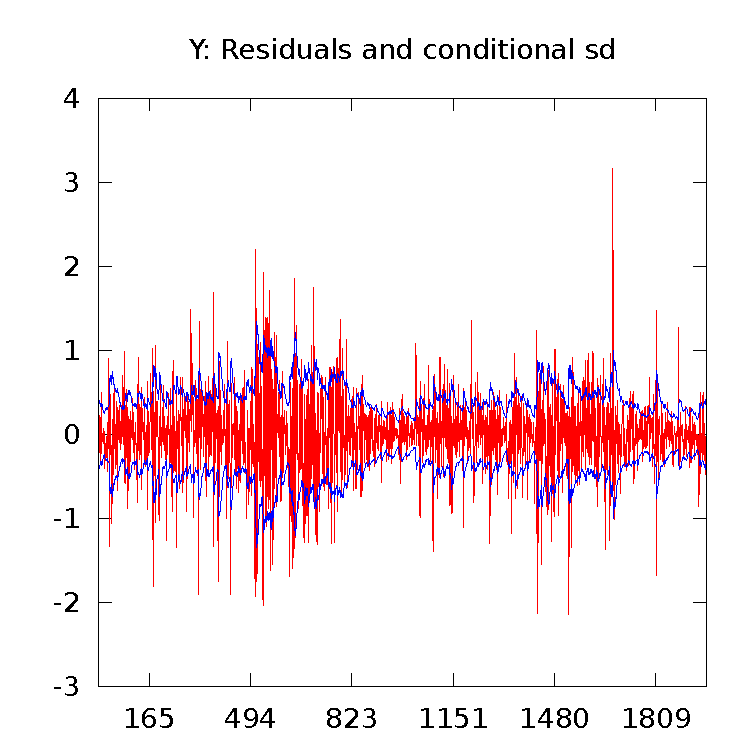
\includegraphics[scale=0.5]{graphs/plot_ex} &
    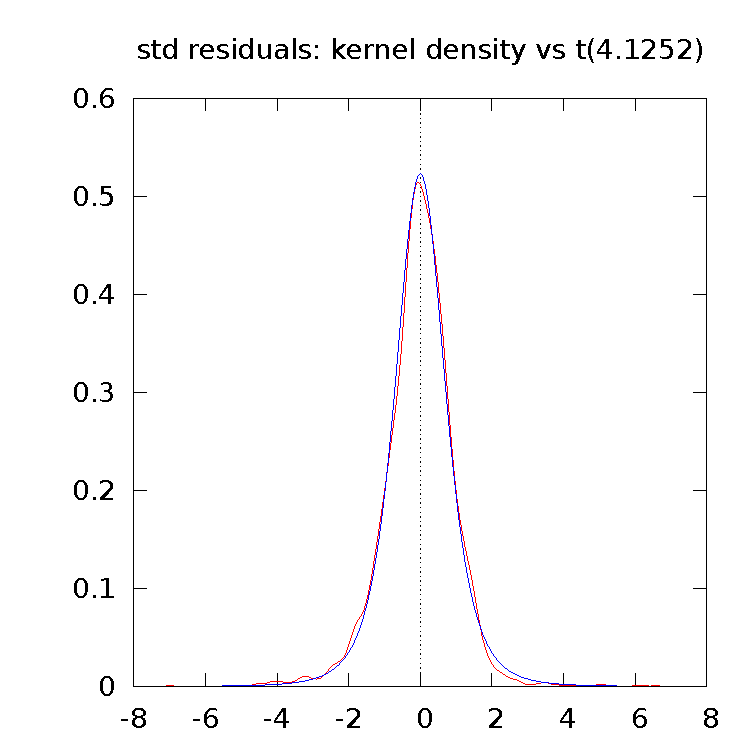
\includegraphics[scale=0.5]{graphs/dplot_ex} \\
    \texttt{gig\_plot} example &
    \texttt{gig\_dplot} example 
  \end{tabular}
  \caption{Example plots}
  \label{fig:ex-plots}
\end{figure}


The \gig\ package provides three built-in functions for plotting the
results of a model: \cmd{gig\_plot}, \cmd{gig\_dplot} and
\cmd{gig\_vfgraph}, which correspond to the ``Time series'',
``Density'' and the ``Forecast'' entries of the ``Plot'' GUI menu (see
subsection \ref{sec:GUI}).

The \cmd{gig\_plot} function produces a plot that is very similar to
the one that \app{gretl}'s native GARCH routine gives you after
estimation, that is a time-plot of the model residuals and the
estimated conditional standard deviation. 

The \cmd{gig\_plot} function, instead, compares the estimated density
of the standardised innovations to their non-parametric kernel
estimate and can be used for judging visually how adequate the choice
of a conditional distribution is.

The following code
fragment exemplifies of their usage in a script; the input code:

\begin{code}
include gig.gfn
open b-g.gdt
epicurus = gig_setup(Y,7,const)
gig_set_dist(&epicurus, 1)
gig_estimate(&epicurus)
gig_plot(&epicurus)
gig_dplot(&epicurus)  
\end{code}
produces the following output
\begin{code}
Model: EGARCH(1,1) [Nelson] (Student's t)
Dependent variable: Y
Sample: 1-1974 (T = 1974), VCV method: Robust

    Conditional mean equation

             coefficient    std. error      z       p-value
  ---------------------------------------------------------
  const      -0.000238229   0.00686306   -0.03471   0.9723 

    Conditional variance equation

             coefficient   std. error     z      p-value 
  -------------------------------------------------------
  omega      -0.220313     0.0623767    -3.532   0.0004   ***
  alpha       0.255802     0.0624886     4.094   4.25e-05 ***
  gamma      -0.0379411    0.0181844    -2.086   0.0369   **
  beta        0.977675     0.0125505    77.90    0.0000   ***

    Conditional density parameters

             coefficient   std. error     z     p-value 
  ------------------------------------------------------
  ni           4.12520      0.402748    10.24   1.28e-24 ***

	Llik:   -986.08927	 AIC:   1984.17853
	BIC:    2017.70544	 HQC:   1996.49706
\end{code}
and the plots shown in Figure \ref{fig:ex-plots}.

The function \cmd{gig\_vfgraph}, instead, is a little more complex: it
takes four arguments. The first one is a matrix with the results of
the simulations used to forecast the variances, such as the one
produced by the \cmd{gig\_var\_fcast} function. The other two are two
scalars indicating how many observation of the in-sample fitted
variants you want in the graph and the width of the coverage region
(between 0 and 1).

\section{Numerical issues}
\label{sec:numerical}

\subsection{\gig\ is slow, especially EGARCH}
Analytical derivatives of the likelihood for APARCH model with normal
innovations were computed by \cite{Laurent}. At present, however,
\gig\ relies on numerical differentiation only for some of the models
it handles\footnote{Note to the reader: we wouldn't feel offended if
  \emph{you} helped with the code for the analytical score, you
  know. Not in the slightest.}. 

An important difference between equation \eqref{eq:aparch} and
\eqref{eq:egarch} is that in the APARCH case the conditional variance
can be written as a linear filter of the $\uhat_{t-i}$ variables,
whereas in the EGARCH formulation you have the $\stdu_{t-i}$
variables, so the EGARCH filter is not linear. Given the way \gig\ is
presently written (and the fact that we haven't coded the analytical
score for EGARCH yet), this implies that EGARCH filtering is much more
time-consuming than APARCH filtering, and as a consequence estimation
times are somewhat longer. We're working on this.

\subsection{The maximisation algorithm fails to converge}

All statistical models that rely on numerical optimisation methods may
suffer from convergence or accuracy problems. In case you encounter
convergence problems, you may want to try the following tricks:
\begin{itemize}
\item Enable the highest level of verbosity in
  \texttt{gig\_estimate()} to see what goes wrong.
\item Rescale your data. Estimation may be sensitive to the scale of
  the dependent variable and/or your explanatory variables. There is
  an internal algorithm to rescale some data ``sensibly'', but is not
  guaranteed to work. Should you encounter convergence problems, it is
  advisable to scale $y_t$ so that its variance is between 0.01 and
  100. A useful thumb rule is that, for example, returns should be
  computed as $r_t = 100 \cdot \Delta \ln P_t$.
\item Try changing the optimisation algorithm via \texttt{set lbfgs}
  or \texttt{set optimizer newton}; see the User's Guide for more details.
\item Try starting the algorithm from a different starting point than
  the default. In order to do this, you must modify the \texttt{coeff}
  element of the model bundle before calling
  \texttt{gig\_estimate}. See the example below.
\end{itemize}


\begin{scode}
include gig.gfn
open b-g.gdt --quiet                    # Bollerslev-Ghysels esample dataset
moo = gig_setup(Y, 3, const)            # GJR, no regressors
gig_set_pq(&moo, 2, 1)                  # set p and q (just for fun)
theta_0 = moo.coeff                     # the automatic starting values
print theta_0                           # have a look at them
gig_estimate(&moo,2)                    # now estimate verbosely
theta_1 = {0; 0.5; 0.2; 0; 0.7; 0.1; 2} # choose another starting point
moo.coeff = theta_1                     # stuff it into the model
gig_estimate(&moo,2)                    # now re-estimate verbosely
\end{scode}

\subsection{The algorithm converges but complains about a singular
  Hessian}

All the items in the previous subsection apply. Moreover, consider
that perhaps your problem \emph{is} ill-conditioned after
all. Conditionally heteroskedastic model can be very picky, especially
with few datapoints. Try similar models and/or slightly different
sample ranges to see what happens.

\subsection{The algorithm converges, but the maximum is outside the
  admissible region!}

In the fuzzy and comfortable world of GARCH(1,1), the constraints
$\alpha > 0$, $\beta \ge 0$ and $\alpha + \beta < 1$ are natural,
because you want your conditional variances $h_t$ to be positive and
finite for all $t$. Note that each of those requirements has a slight
different reason: for example, $\alpha = 0$ would make the model
underidentified, so it's an absolute must. On the other hand, the
requirement $\alpha + \beta < 1$ applies to the \emph{true}
parameters, whereas their \emph{estimates} may happily violate that
requirement in a finite sample: for example, the point in the
parameter space which maximises the likelihood may well be outside the
admissible range just because your dataset ends with a massive
volatility burst. A similar argument goes for models with $q>1$; the
second-lag ARCH parameter $\alpha_2$, for instance, must be positive to
ensure that $h_t$ can never be negative, but in a finite sample you
can have that the sequence of conditional variances that maximise the
likelihood is the one associated with a small negative value for
$\alpha_2$.

Besides, you should also handle the case, which is frequent in
practice, of parameters which go outside the admissible region during
maximisation and eventually go back into it because the maximum is
inside that region after all.

In such a situation, surely you wouldn't want the software to hide the
problem from you, so just printing out something like 
\begin{code}
  I'm sorry, your estimates are outside the admissible region
\end{code}
would be a pathetically patronising decision from the software (that
is, from us). In our opinion, the best policy is to treat these
results for what they are: a finite-sample oddity if your model is
right or (more likely) an indication that perhaps your model wasn't
the best choice after all.

So, the current state of things in \gig\ is: no constraints are put on
the parameters. In the future, we'll issue a warning if the algorithm
stops at some unorthodox point. This is easy for a GARCH(1,1) model:
for GARCH($p$,$q$) models, this is more complex, but still
possible\footnote{Again, a little help with the coding of the
  Nelson-Cao conditions would not be unwelcome.}
\citep{NelCao92}. However, it's not clear what to do with models with
exogenous variables in the volatility equation or non-GARCH models. We
are not aware of a generalisation of the Nelson-Cao conditions for the
APARCH model; pointers would be appreciated, if any of you know of
any.

\bibliography{gig}

%\clearpage
\appendix

\section{List of functions}
\label{sec:syntax}
\subsection{Model setup}
\label{sec:gig_setup}

\begin{funcdoc}{gig\_setup(series depVar, scalar type, list X, 
			  list varX, scalar ARlags)}
\begin{enumerate}
\item a series containing $y_t$, the dependent variable \textbf{(required)}
\item a scalar for the model type (see Table \ref{tab:modelcodes},
  left-hand side)
\item a list with the exogenous variables in the mean equation: in
  terms of eq.~\eqref{eq:espdef}, the $x_t$ variables. Lags of the
  dependent variable, if any, must be included in this list. (Default:
  \texttt{null})
\item a list with the exogenous variables in the variance equation: in
  terms of eq.~\eqref{eq:vareq}, the $z_t$ variables. A constant term
  is automatically included if absent. (Default: \texttt{null})
\item a scalar, holding the number of autoregressive terms in the mean
  equation. (Default: 0)
\end{enumerate}
\end{funcdoc}

\begin{funcdoc}{gig\_set\_dist(bundle *b, int code)}
\begin{enumerate}
\item the address of a model bundle created via \texttt{gig\_setup}
  \textbf{(required)}
\item a scalar for the conditional density function (see Table \ref{tab:modelcodes},
  right-hand side)
\end{enumerate}
\end{funcdoc}

\begin{funcdoc}{gig\_set\_pq(bundle *b, int p, int q)}
\begin{enumerate}
\item the address of a model bundle created via \texttt{gig\_setup}
  \textbf{(required)}
\item  $p$, the GARCH order (between 0 and 2, default 1)
\item  $q$, the ARCH order (minimum 1, default 1)
\end{enumerate}
\end{funcdoc}

\begin{funcdoc}{gig\_set\_vcvtype(bundle *b, string s)}
\begin{enumerate}
\item the address of a model bundle created via \texttt{gig\_setup}
  \textbf{(required)}
\item  a string: ``Hessian'', ``OPG'' or ``Sandwich'';
  \textbf{(required)}. Note that
  \begin{enumerate}
  \item the function is case-insensitive, so ``opg'' and ``OPG''
    produce the same effect;
  \item other strings than the ones listed above produce no effect.
  \end{enumerate}
\end{enumerate}
\end{funcdoc}

\begin{funcdoc}{gig\_set\_vQR(bundle *b, boolean on\_off)}
\begin{enumerate}
\item the address of a model bundle created via \texttt{gig\_setup}
  \textbf{(required)}
\item 1 to activate the QR decomposition for variance regressors, 0 to
  de-activate
\end{enumerate}
\end{funcdoc}

\subsection{Estimation}
\label{sec:syntax_estim}

\begin{funcdoc}{gig\_estimate(bundle *b, int verbose[0:2:1])}

General estimation function. % It returns a matrix with the estimation
% results stored in packed form (see appendix \ref{sec:output_struct}).
Its arguments are:
\begin{enumerate}
\item the address of a model bundle created via \texttt{gig\_setup}
  \textbf{(required)}
\item a verbosity switch, from 0 to 2. (Default: 1)
\end{enumerate}
\end{funcdoc}

\begin{table}[htbp]
  \centering
  \begin{tabular}{rl|rl}
    \hline
    \textbf{Code} & \textbf{Model Type} & \textbf{Code} & \textbf{Density Type} \\
    \hline
    0 & ARCH & 0 & Normal (default) \\
    1 & GARCH (default) & 1 & Student's $t$ \\
    2 & Taylor/Schwert GARCH & 2 & GED\\
    3 & GJR & 3 & Skewed $t$ \\
    4 & Zakoian's TARCH & 4 & Skewed GED \\
    5 & NARCH \\
    6 & APARCH \\
    7 & EGARCH \\
    \hline
    \hline
  \end{tabular}
  \caption{Model type/density function codes}
  \label{tab:modelcodes}
\end{table}

\subsection{Output}
\label{sec:syntax_output}

Note: these functions assume that the bundle they refer to contain a
model that has already been estimated. No checks is performed.

\begin{funcdoc}{gig\_print(bundle *b, scalar verbose)}
  Prints out a model.
\end{funcdoc}

\begin{funcdoc}{gig\_plot(bundle *b)}
  Plots the residuals/conditional SE graph.
\end{funcdoc}

\begin{funcdoc}{gig\_dplot(bundle *b)}
  Plots the estimated density of the standardized residuals versus its
  nonparametric estimate.
\end{funcdoc}

\clearpage

\section{Bundle elements}
\label{sec:bundle_struct}
\begin{footnotesize}
\begin{tabular}{rlp{0.7\textwidth}}
  \hline
  \textbf{Name} & \textbf{Type} & \textbf{Purpose} \\
  \hline
  \multicolumn{3}{c}{Model descriptors} \\
  \hline
  \texttt{type} & scalar & model type (as per Table \ref{tab:modelcodes})\\
  \texttt{AR} & scalar & AR order (mean equation) \\
  \texttt{p} & scalar & GARCH order\\
  \texttt{q} & scalar & ARCH order\\
  \texttt{cdist} & scalar & conditional density (as per Table \ref{tab:modelcodes})\\
  \texttt{mlistX} & matrix & list of mean regressors \\
  \texttt{vlistX} & matrix & list of variance regressors \\
  \texttt{mk} & scalar & number of mean regressors \\ 
  \texttt{vk} & scalar & number of variance regressors\\
  \texttt{nobs} & scalar & number of observations \\
  \texttt{t1} & scalar & first observation used \\
  \texttt{t2} & scalar & last observation used \\
  \hline
  \multicolumn{3}{c}{Strings} \\
  \hline
  \texttt{depvarname} & string & dependent variable name\\
  \texttt{mXnames} & string    & mean regressors names \\
  \texttt{vXnames} & string    & variance regressors names \\
  \hline
  \multicolumn{3}{c}{Data} \\
  \hline
  \texttt{y} & series  & dependent variable \\
  \texttt{mX} & matrix & mean regressors \\
  \texttt{vX} & matrix & variance regressors\\
  \texttt{s2} & scalar & sample variance of the OLS residuals of $y$ on $X$
  \\
  \hline
  \multicolumn{3}{c}{Estimation parameters} \\
  \hline
  \texttt{scale} & scalar & auto-scaling (used internally) \\
  \texttt{vcvtype} & scalar & method for computing the covariance
  matrix: 0 = Sandwich (default), 1 = Hessian, 2 = OPG\\
  \texttt{inipar} & matrix  & Starting values for BFGS \\
  \texttt{active} & matrix  & indicates which elements of the parameter
  vector are active during ML estimation\\
  \texttt{vX\_QR} & scalar  & Toggles QR decomposition for variance regressors\\
  \hline
  \multicolumn{3}{c}{Estimation results} \\
  \hline
  \texttt{errcode} & scalar & error code from BFGS (0 = ok)\\
  \texttt{coeff} & matrix & coefficients \\
  \texttt{stderr} & matrix & std. deviations \\
  \texttt{vcv} & matrix & covariance matrix \\
  \texttt{uhat} & series & residuals \\
  \texttt{h} & series & conditional variance \\
  \texttt{stduhat} & series & standardised residuals \\
  \texttt{criteria} & matrix & information criteria\\
  \hline
  \hline
\end{tabular}
\end{footnotesize}

\clearpage

NOTA BENE: For APARCH models, the order in which the estimated
parameters are stored in the \texttt{coeff} matrix is the following: 
\begin{enumerate}
\item Conditional mean parameters
\item $\omega_0 \ldots \omega_k$, where $k$ is the number of variance
  regressors; the constant in equation \eqref{eq:aparch} is here.
\item $\alpha_1 \ldots \alpha_q$
\item $\gamma_1 \ldots \gamma_q$; if the model contains ``leverage''
  terms (otherwise, \emph{eg} with the plain GARCH model, you have
  zeros here)
\item $\beta_1 \ldots \beta_p$
\item parameters for the conditional density: for example, degrees of
  freedom $\nu$ for Student's $t$.
\end{enumerate}
\end{document}


%%% Local Variables: 
%%% mode: latex
%%% TeX-master: t
%%% End: 

